\documentclass[tikz]{standalone}
\usepackage{pgfplots}
\pgfplotsset{compat=1.18}
\begin{document}
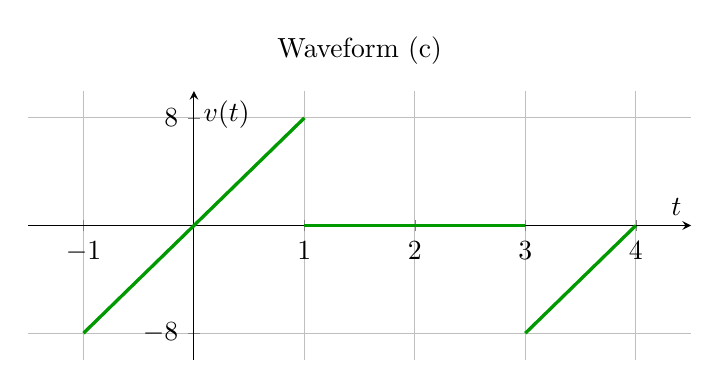
\begin{tikzpicture}
\begin{axis}[
    axis lines = middle,
    xlabel = {$t$},
    ylabel = {$v(t)$},
    xmin = -1.5, xmax = 4.5,
    ymin = -10, ymax = 10,
    xtick = {-1, 0, 1, 2, 3, 4},
    ytick = {-8, 0, 8},
    grid = both,
    width=10cm, height=5cm,
    title = {Waveform (c)}
]
\addplot[green!60!black, very thick, domain=-1:1, samples=2] {8*x};
\addplot[green!60!black, very thick, domain=1:3, samples=2] {0};
\addplot[green!60!black, very thick, domain=3:4, samples=2] {8*(x-4)}; % Start next period
\end{axis}
\end{tikzpicture}
\end{document}
